% Template for Cogsci submission with R Markdown

% Stuff changed from original Markdown PLOS Template
\documentclass[10pt, letterpaper]{article}

\usepackage{cogsci}
\usepackage{pslatex}
\usepackage{float}
\usepackage{caption}

% amsmath package, useful for mathematical formulas
\usepackage{amsmath}

% amssymb package, useful for mathematical symbols
\usepackage{amssymb}

% hyperref package, useful for hyperlinks
\usepackage{hyperref}

% graphicx package, useful for including eps and pdf graphics
% include graphics with the command \includegraphics
\usepackage{graphicx}

% Sweave(-like)
\usepackage{fancyvrb}
\DefineVerbatimEnvironment{Sinput}{Verbatim}{fontshape=sl}
\DefineVerbatimEnvironment{Soutput}{Verbatim}{}
\DefineVerbatimEnvironment{Scode}{Verbatim}{fontshape=sl}
\newenvironment{Schunk}{}{}
\DefineVerbatimEnvironment{Code}{Verbatim}{}
\DefineVerbatimEnvironment{CodeInput}{Verbatim}{fontshape=sl}
\DefineVerbatimEnvironment{CodeOutput}{Verbatim}{}
\newenvironment{CodeChunk}{}{}

% cite package, to clean up citations in the main text. Do not remove.
\usepackage{cite}

\usepackage{color}

% Use doublespacing - comment out for single spacing
%\usepackage{setspace}
%\doublespacing


% % Text layout
% \topmargin 0.0cm
% \oddsidemargin 0.5cm
% \evensidemargin 0.5cm
% \textwidth 16cm
% \textheight 21cm

\title{Conceptual and prosodic cues in child-directed speech can help children
learn disjunction meaning}


\author{{\large \bf Masoud Jasbi} \\ \texttt{masoudj@stanford.edu} \\ Department of Linguistics \\ Stanford University \And {\large \bf Akshay Jaggi} \\ \texttt{ajaggi@stanford.edu} \\ Department of Linguistics \\ Stanford University \And {\large \bf Michael C. Frank} \\ \texttt{mcfrank@stanford.edu} \\ Department of Psychology \\ Stanford University }

\begin{document}

\maketitle

\begin{abstract}
Ambiguity poses a challenge to children's acquisition of word meaning.
For example, a disjunction such as \emph{A or B} can be interpreted as
inclusive (A or B, or both) or exclusive (A or B, not both). Linguistic
studies suggest that the core meaning of \emph{or} is inclusive and that
the exclusive interpretation is the result of other (extra-semantic)
factors such as pragmatic reasoning. However, research in langauge
acquisition shows that the majority of \emph{or} examples children hear
are exclusive, yet children interpret \emph{or} as inclusive in
comprehension tasks. This raises a larning puzzle: how can children
quickly learn what they rarely hear? We argue that children can use the
conceptual and prosodic cues cues to exclusivity in child-directed
speech to learn the interpretation of a disjunction from a few examples.

\textbf{Keywords:}
language acquisition; word learning; logical words; conjunction,
disjunction.
\end{abstract}

\section{Introduction}\label{introduction}

The social media company LADbible reported the following in a tweet:
``James Bond producer says next 007 could be black \textbf{or} a
woman''. A twitter user named Robert responded sarcastically with: ``if
only women could be black!'' What in the producer's speech gave the
impression that the next 007 could not be both black \textbf{and} a
woman? The word \emph{or}. A disjunction like ``A or B'' is associated
with two interpretations: \textbf{inclusive}, and \textbf{exclusive}.
``A or B'' is inclusive when it is interpreted as ``A or B \textbf{or
both}''. This is probably what LADbible meant when reporting the James
Bond producer. However, ``A or B'' can also be exclusive: ``A or B, but
\textbf{not both}''. Robert's response shows that he had an exclusive
interpration of \emph{or}. What factors determine the interpretation of
\emph{or} and how do children learn its meaning given the ambiguity it
can give rise to?

A large body of research in linguistics and philosophy in the past 50
years has created a common consensus on the meaning of \emph{or} (see
Aloni (2016)). Data on the interpretation of disjunction across
different sentences, contexts, and even languages show that the core
meaning of disjunction words such as \emph{or} is \textbf{inclusive}.
This is similar to the definition of disjunction in formal logics. The
\textbf{exclusive} interpretation of \emph{or} is the result of
enhancing its inclusive semantics via other (extra-semantic) factors
such as intonation (Pruitt \& Roelofsen, 2013), inconsistency of the
options (Geurts, 2006), and pragmatic reasoning over the speaker's
choice of \emph{or} instead of \emph{and} (Grice, 1975). Therefore,
interpreting a disjunciton is a complex process that needs to take into
account the meaning of \emph{or} as well as different structural and
contextual factors that accompany it. How do we, as children, learn such
a complex interpretive system?

There are two accounts of children's acquisition of disjunciton: a
\textbf{constructivist} account, and 2. a \textbf{nativist} account.
Under the constructivist account, children learn the meaning of
\emph{or} by paying attention to how parents use it in different
contexts. They form usage-rules and expand their usage repertoire as
they grow up. The prediction is that children's production of \emph{or}
is slow and gradual, mirroring what they hear from parents. Morris
(2008) found that \emph{and} is about 13 times more frequent than
\emph{or} in parents' speech to children. As predicted by the
constructivist account, Morris (2008) reported that children also learn
to produce \emph{and} much more quickly than \emph{or}. They reach the
adult rate of \emph{and} at age 3 while for \emph{or} there is a gradual
increase in production, possibly reaching the adult level at ages 5 or
6. The faster acquisition of \emph{and} is consistent with the
constructivist theory that emphasizes the role of usage frequency in
children's linguistic development. Morris (2008) also reported that the
majority of \emph{or} examples children hear are exclusive. He argued
that consistent with the constructivist account, the majority of
\emph{or}'s children produce are also exclusive. Therefore, the
inclusive semantics of \emph{or} is developed after the exclusive
interpretation.

However, several comprehension studies of \emph{or} in different
linguistic contexts show that children as young as three-years old
interpret \emph{or} as inclusive disjunction (Crain, 2012). This is
surprising given Morris (2008)`s finding that the majority of \emph{or}
examples children hear are exclusive. How do children learn the
interpretation of disjunction as inclusive if they rarely hear it? We
call this the \textbf{learning puzzle of disjunction}. Crain (2012)
suggests that instead of learning from the parents' usage of \emph{or},
children rely on the innate knowledge that the the disjunciton operator
in their native language must have an inclusive meaning. This nativist
account predicts that \emph{or} is learned relatively quickly and
accurately by children.

Here we present an alternative answer that provides a synthesis between
the nativist and constructivist accounts. We show that children can use
regularities in parents' usage of \emph{or} to learn the interpretation
of disjunction from a handful of examples. In study 1, we use a large
scale corpus study of parents and children's speech to show that both
\emph{and} and \emph{or} appear relatively quickly in children's speech
and reach the adult rate by the age 4. This finding is consistent with
the comprehension studies that show children have an adult-like
understanding of these words by the age four. In study 2, we replicate
Morris (2008)'s finding that the majority of \emph{or} examples in
child-directed speech have an exclusive interpretation. However, we also
show that these exclusive interpretations correlate systematically with
two factors external to \emph{or}: intonation and consistency of the
options. Exclusive interpretations are either inconsistent in nature
(e.g.~clean or dirty) or carry a distinct rise-fall intonation. We show
that setting aside these cases, the interpretation of a disjunction is
inclusive.

We argue that if children track the interpretive cues that accompany a
disjunction, they can tease apart the role of the word \emph{or} from
factors that accompany and enhance it to shape the exclusive
interpretation. This way children can discover that exclusivity
corrleates with rise-fall intonation and inconsistent options, while
\emph{or} itself does not exclude the option of both disjuncts being
true. We implement this novel account in a decision-tree that correctly
learns to predict the interpretation of a disjunction with 80\% accuracy
after only a few examples. Our results show that the richness and
systematicity of children's linguistic input allows rapid acquisition of
disjunction with no need for an innate assumptions specific to the
meaning of disjunction. We discuss the important implications of this
work for the theories of word learning in the last section.

\section{Study 1: Corpus Study}\label{study-1-corpus-study}

First, we conducted an exploratory and large scale investigation of
\emph{and} and \emph{or} productions in parents and children. The goal
of the study was to find out when children start producing these words
and when they reach the adult rate of production. We conclude that
children start producing \emph{and} around 1.5 or 2 years of age, and
\emph{or} between the ages of 2 and 3. They reach the adult rate of
production for \emph{and} around 3 and for \emph{or} around 4 or
possibly earlier.

\subsection{Methods}\label{methods}

We accessed the Child Language Data Exchange System
(\href{https://childes.talkbank.org/}{CHILDES}, MacWhinney (2000)) via
the online platform \href{http://childes-db.stanford.edu/}{childes-db}
and its associated R package childesr (Sanchez et al., in prep). We
extracted all instances of \emph{and} and \emph{or} from the English
corpora (ENG-NA and ENG-UK). We limited our analysis to the data between
one and six years because there is scarce data outside this age range.
We computated the relative frequency of connective production by
dividing the total number of \emph{and}/\emph{or} in the speech of
fathers, mothers, and children at a particular age by the total number
of words spoken at that age. We present the relative frequency as parts
per thousand.

\begin{CodeChunk}
\begin{figure}[t]
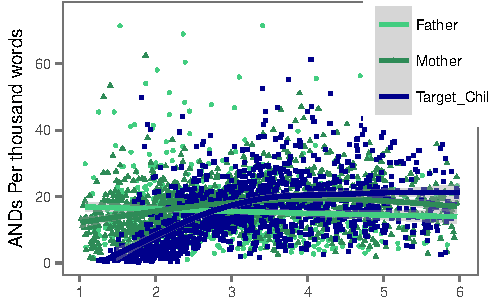
\includegraphics{figs/OverallConnectivePlots-1} 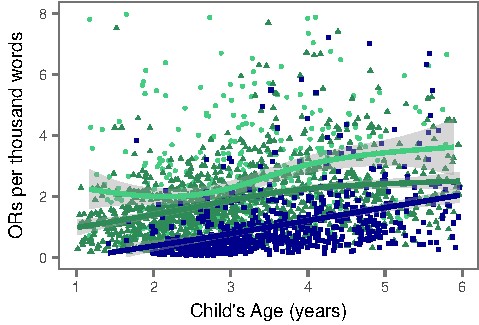
\includegraphics{figs/OverallConnectivePlots-2} \caption[The relative frequency of AND (top) and OR (bottom) per thousand words in the speech of fathers, mothers, and children between the ages of 1 and 6]{The relative frequency of AND (top) and OR (bottom) per thousand words in the speech of fathers, mothers, and children between the ages of 1 and 6.}\label{fig:OverallConnectivePlots}
\end{figure}
\end{CodeChunk}

\subsection{Results}\label{results}

\begin{CodeChunk}
\begin{figure*}[t]

{\centering 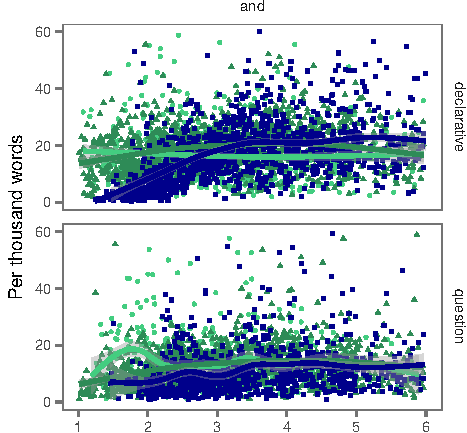
\includegraphics{figs/byspeechActPlots-1} 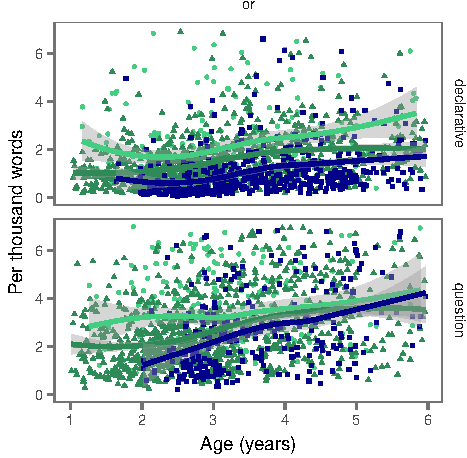
\includegraphics{figs/byspeechActPlots-2} 

}

\caption[The relative frequency of AND (left) and OR (right) per thousand words in delcaratives and questions in the speech of fathers, mothers, and children between the ages of 1 and 6]{The relative frequency of AND (left) and OR (right) per thousand words in delcaratives and questions in the speech of fathers, mothers, and children between the ages of 1 and 6.}\label{fig:byspeechActPlots}
\end{figure*}
\end{CodeChunk}

In figure 1, we show the relative frequencies of \emph{and} and
\emph{or} in the speech of parents and children between one and six
years. It is important to note that the y-axes for \emph{and} vs.
\emph{or} show different ranges. This is due to the big difference in
the relative frequencies of \emph{and} and \emph{or}. In the speech of
parents, \emph{and} is produced around 20 times per thousand words while
\emph{or} is only produced around 2 times per thousand words. This
confirms previous findings that \emph{or} is much less frequent in child
directed speech than a similar funciton word such as \emph{and}.

\emph{And} and \emph{or} seem to show different developmental
trajectories in the speech of children. For \emph{and}, there is a rapid
increase in its production between the ages of 1.5 and 3 before it
reaches the adult rate around the age 3 and stay at that level until the
age 6. For \emph{or}, on the other hand, we see a slow incrase from the
age 2 until the age 6 when it reaches the adult rate. This difference in
the development of \emph{and} \& \emph{or} production was attributed to
the frequency of these items in child-directed speech. Since \emph{and}
is much more frequent than \emph{or}, it is learned much faster than
\emph{or}. Morris (2008) argued that such patterns support the
item-based and usage-based acquisition of logical words.

However, the analysis above does not control for other factors that can
affect the production of words by children. An important factor to
control for is the development of speech acts. While content words such
as \emph{dog} or \emph{chair} may appear freely in different types of
speech acts, function words are highly constrained by the type of speech
acts they can appear in. For example, it is reasoable to assume that
question words such as \emph{how} and \emph{why} are much more likey to
occur in questions than statements (declaratives). If parent-child
interaction is such that parents ask more questions than children, it is
not surprising to find higher rates of \emph{how} and \emph{why}
production in parents than children. Therefore, it is important to
control for the speech act a function word appears in.

Figure 2 shows the relative frequencies of \emph{and} and \emph{or} in
questions vs.~declaratives, in the speech of parents and children
between one and six years. Here, the relative frequency is computed by
dividing the total number of \emph{and}/\emph{or} in a
question/declarative in the speech of fathers, mothers, and children at
a particular age, by the total number of words in a question/declarative
spoken at that age. As before, we present the relative frequency as
parts per thousand.

The results show similar developmental trajectories for the production
of \emph{and} and \emph{or} in children. For both words, there is a
relatively rapid incease in their frequency between the ages of 2 and 4
before reaching the parent rate at the age of 4 and staying at that rate
until the age of 6. This pattern of production is consistent with the
nativist observations that the acquisition of \emph{and} and \emph{or}
is rapid and that children have an adult-like comprehension of these two
connectives at the age 4.

\subsection{Summary}\label{summary}

In this study we found that \emph{and} is a lot more frequent than
\emph{or} in child directed speech. Looking at the relative frequency of
\emph{and} and \emph{or} between the ages of 1 and 6, it appeared as if
children show radically different developmental trajectories for these
two connectives. Children's production of \emph{and} seemed to sharply
increase around the age 1.5 and reach the adult rate around age 3 while
\emph{or} production increased slowly and linearly until it reached the
adult rate at age 6. However, we showed that this discrepency is to a
large part due to the distribution of function words in different speech
acts. Since \emph{or} is more frequent in questions and children produce
fewer questions than parents, the frequency of \emph{or} in children's
speech is underestimated if we normalize by the total number of words
they produce. Instead, when we look at the production of \emph{and} and
\emph{or} in specific speech acts - declaratives and questions - and
normalize by the total number of words produces in each speech act, we
see that \emph{and} and \emph{or} show similar developmental patterns.
We argue that the developmental trajectory of \emph{and} \& \emph{or} is
best described as a quick increase in production between the ages of 2
and 4 and staying around the parents' rate between the ages 4 and 6.
This is compatible with the comprehension studies which suggest children
understand \emph{and} and \emph{or} by the age four.

\section{Study 2: Annotation Study}\label{study-2-annotation-study}

Study 1 showed that even though \emph{or} is not very frequent in
child-directed speech, children learn and produce it relatively quickly
and reach the adult rate around the age 4. In study 2, we conducted a
detailed and small-scale investigation of \emph{or} productions in
child-directed speech. The goal of the study was to find out how
children learn the meaning of \emph{or} from such little data. We
conclude that children hear significantly more exclusive uses of
\emph{or} supporting Morris (2008)'s findings. However, we also find
that the exclusive uses of \emph{or} are rich in structures that index
the exclusive interpretation. These indicative structures include
rise-fall intonation and consistency of the options. Exclusive
interpretations are either inconsistent in nature (e.g.~clean or dirty)
or carry a distinct rise-fall intonation. We then show that a decision
tree model can learn to accurately (\textgreater{}80\%) predict
exclusivity using this information after seeing few (\textless{}20)
examples. Instances of \emph{or} without these indices are most likely
interpreted as inclusive.

\subsection{Methods}\label{methods-1}

We accessed the Providence corpus via CHILDES ({\textbf{???}}). We
extracted all instances of \emph{or} along with the two utterances
before and after to provide context. We annotated the examples for four
major categories: 1. Interpretation 2. Intonation and 3. Conceptual
consistency. Table 1 shows shows these categories along with their
subcategories and an example for each subcategory. The first category -
disjunction interpretation - was our dependent measure. Annotators
listened to a disjunciton like ``A or B'' and decided whether the
speaker intended to imply ``not both A and B'' (exlcusive) or ``possibly
both A and B'' (inclusive). For the second category - intontation -
annotators listened to the sentence containing disjunction and decided
whether the intonation contour on the disjunciton is rise-fall, rise, or
flat. It is difficult to convey these intonation types in writing here
but Table 1 includes examples that are prototypically read aloud with
the intonation contour they are subcategorized as.

Finally, for conceptual consistency, annotators decided wether the
propositions that make up the disjunction are inconsistent. For example,
a disjunctive statement such as ``The ball is in my room or your room''
denotes two propositions: 1. The ball is in my room 2. The ball is in
your room. Regardless of the connective used for these propositions, the
propositions themselves refer to inconsistent states of affairs: they
cannot be both true at the same time. In such cases, the inclusive
meaning is simply not available due to the nature of the propositions
themselves and not the interpretation of the connective. Our annotators
used the following diagnostic to decide the consistency of the
disjuncts: Two disjuncts were marked as inconsistent if replacing the
word \emph{or} with \emph{and} produced a contradiction. For example
``The ball is in my room and your room'' is contradictory. The ball
cannot be in two positions at the same time. It is important to note
here that this is a particularly strict diagnostic. In many cases, the
possibility of both propositions being true is ruled out based on prior
knowledge and expectations of the situation. For example, when asking
people whether they would like tea or coffee, it is often assumed that
people choose one or the other. However, wanting to drink both tea and
coffee is not conceptually inconsistent. It is just very unlikely. Our
annotations of consistency are very conservative in that they consider
such unlikely cases as consistent.

\begin{table}[H]
\centering
\begin{tabular}{lll}
 Category & Subcategory & Examples \\ 
  \hline
Interpretation & Exclusve & Wanna stay or go? \\ 
   & Inclusive & Anything to eat or drink? \\ 
   \hline
Intonation & Flat & I'll get tea or coffee. \\ 
   & Rise & Anything to eat or drink? \\ 
   & Rise-Fall & Wanna stay or go? \\ 
   \hline
Consistency & Consistent & I'll get tea or coffee. \\ 
   & Inconsistent & Wanna stay or go? \\ 
  \end{tabular}
\caption{Annotation categories and examples.} 
\end{table}

We would also like to add that both intonation and conceptual
conisistency were chosen based on previous linguistic research that
showed their role in the interpretation of disjunction. In an
experimental study, ({\textbf{???}}) showed that a rise-fall intonation
results in an exclusive interpretation in adults. Geurts (2006) had
already emphasized the fact that in many cases, exclusivity is due to
the nature of the propositions being communicated and not the
interpretation of \emph{or}. This study shows to what extant these
factors can help language acquisition.

Fingally, to test inter-rater reliability, the two raters annotated the
same 240 utterances. The interrater reliability was calculated over 8
iterations of 30 examples each. Training only completed after 3
consecutive iterations with reliability over 0.7 for all categories.

\begin{CodeChunk}
\begin{figure}[b]

{\centering 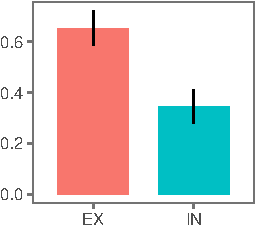
\includegraphics{figs/interpretation-1} 

}

\caption[Proportion of exclusive and inclusive interpretations of disjunciton in child-directed speech]{Proportion of exclusive and inclusive interpretations of disjunciton in child-directed speech. Error bars represent bootstrapped 95\% confidence intervals}\label{fig:interpretation}
\end{figure}
\end{CodeChunk}

\subsection{Results}\label{results-1}

\begin{CodeChunk}
\begin{figure*}[t]

{\centering 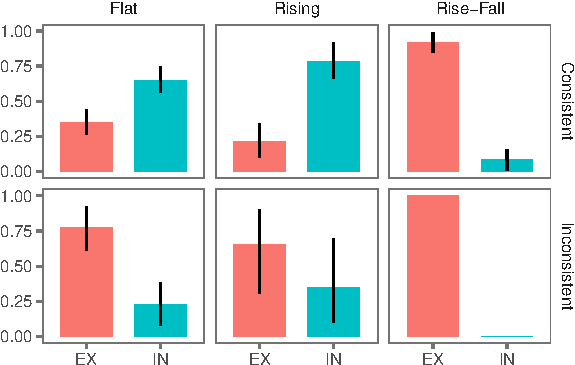
\includegraphics{figs/interpretationByIntonationAndConsistency-1} 

}

\caption[Distribution of exclusive and inclusive interpretations broken down by intonation and consistency]{Distribution of exclusive and inclusive interpretations broken down by intonation and consistency. Error bars represent bootstrapped 95\% confidence intervals}\label{fig:interpretationByIntonationAndConsistency}
\end{figure*}
\end{CodeChunk}

First, similar to Morris (2008), we found that the majority of \emph{or}
examples in CDS receive an exclusive interpretation (\(\sim\)\%65).
Figure 3 shows this difference in distribution. However, the rate of
exclusive interpretations change systematically when we break the data
down by prosody and consistency (Figure 4). Given a rise-fall intonation
contour, a disjunction is almost always interpreted as exclusive.
Similarly, if the propositions are inconsistent, the disjunction is most
likely interpreted as excluisive. When either of these two features are
absent, a disjunction is more likely to receive an inclusive
interpretation.

A mixed-effects binomial logistic regression using the pakcage \{lme4\}
(Bates, Maechler, Bolker, Walker, \& others, 2014) in R with the fixed
effects of intonation and consistency, as well as the random effects for
children found both intonation and consistency significant in
interpreting disjunctions. Disjunctions were more likely to be
interpreted as exlclusive if they received a rise-fall intonation
(\(\beta\)=-3.79, \(z\)=1.66, \(p < 0.001\)) or if they were
inconsistent(\(\beta\)=-2.2, \(z\)=2.08, \(p < 0.001\)). Disjunctions
were more likely to be interpreted as inclusive if they were consistent
and received a rising (\(\beta\)=0.58, \(z\)=0.24, \(p < 0.001\)) or
flat intonation (\(\beta\)=0.38, \(z\)=0.27, \(p < 0.001\)).

\begin{CodeChunk}
\begin{figure}[H]

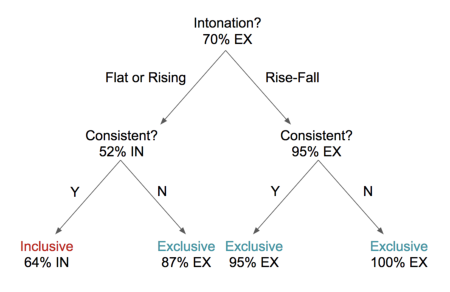
\includegraphics{figs/treeDiagram-1} \hfill{}

\caption[Optimal decision tree training on 200 datapoints]{Optimal decision tree training on 200 datapoints. Intonation $>$ 1.5 are rise-fall while intonation $<$ 1.5 are flat or rising. Consistency $>$ 0.5 are consistent while consistency $<$ 0.5 are  inconsistent. When *or* has neither rise-fall nor inconsistent disjuncts, it is marked inclusive. Otherwise, exclusive.}\label{fig:treeDiagram}
\end{figure}
\end{CodeChunk}

Next, using Sci-kit Learn's Decision Tree Module (Pedregosa et al.,
2011), we built a predictive model to train on annotated \emph{or}
utterances and predict the exclusivity of unseen \emph{or} utterances
(annotated for intonation and consistency). Averaged over 100 trials and
training on 200 examples, the average accuracy of a binary tree was
83\%. More remarkably, the tree achieved an average of 80\% accuracy
after training on only 20 examples. The success of such a simple tree
indicates that children could use a simple model to rapidly learn the
exclusive interpretation of \emph{or} from little data.

\begin{CodeChunk}
\begin{figure}[H]

{\centering 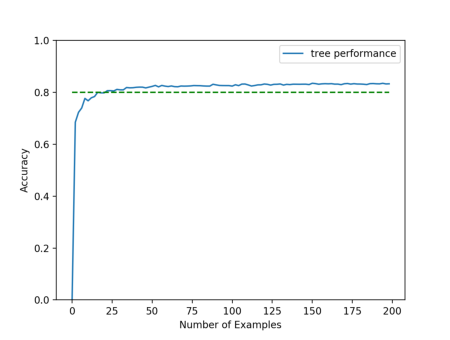
\includegraphics{figs/learningCurve-1} 

}

\caption[Decision Tree Accuracy as a function of number of examples seen]{Decision Tree Accuracy as a function of number of examples seen}\label{fig:learningCurve}
\end{figure}
\end{CodeChunk}

\subsection{Summary}\label{summary-1}

In study 2, we confirm Morris (2008)'s finding that exclusive
interpretations of \emph{or} are far more common than inclusive
interpretations. However, we also show that the majority of these
exclusive interpretations coincide with systematic indicators.
Disjunctions that are accompanied by rise-fall intonation or
inconsistent disjuncts are far more likely to be exclusive. Disjunctions
that do no bear these features are more likely to be inclusive.
Accounting for these external factors, a simple decision tree can
rapidly learn to predict the exclusive interpretation of the
disjunction.

\section{Discussion}\label{discussion}

Studies presented in this paper resolve two puzzles in children's
acquisition of disjunction. First, previous studies suggested a
discrepency between children's production of \emph{or} and their
comprehension. Comprehension studies showed that children have an
almost-adult-like interpretation of \emph{and} and \emph{or} at around
the age 4. However, production studies suggested that \emph{and} is
learned and produced quickly while children have difficuly reaching the
adult rate of production for \emph{or}. Study 1 showed that when we
control for the environments (speech acts) that these connectives are
suitable for, we observe that both \emph{and} and \emph{or} are learned
relatively quickly and produced at an adult rate around the age 4. This
is compatible with the comprehension studies that show 3-to-5-year-olds
understand the meaning of \emph{or} as inclusive disjunction and
\emph{and} as conjunction.

The second puzzle that this study addressed was the (apparent)
discrepency between what they hear from parents and the knowledge they
manifest in comprehension studies. Previous studies showed that the
majority of \emph{or} examples children hear receive an exclusive
interpretation, yet in comprehension tasks they interpret \emph{or} as
inclusive disjunction. Study 2 showed that even though the majority of
\emph{or} examples are exclusive, this exclusivity is due to prosodic
and conceptual properties of the disjunction and not \emph{or} itself.
We showed when we break down interpretations of disjunction in
child-directed speech by prosody and concpetual consistency, the vast
majority of exclusive interpretations are either inconsistent
conceptually (e.g.~clean or dirty) or are accompanied by a distinctive
rise-fall intonation. Otherwise, a disjunction that does not bear these
properties is more likely to be interpreted as inclusive. This finding
suggests that if children break down disjunction interpretations by cues
that accompany them, they can learn the adult like interpretation of
disjunction from child-directed speech. We showed that a decision tree
can use prosody and conceptual consistency to identify the correct
interpretation using less than 20 examples.

The account presented in this paper has important implications for the
theories of form-meaning mapping in general and more specifically
theories of function word acquisition. Form-meaning mapping in child
language acquisition is often construed as the task of associating a
novel and isolated form such as \emph{gavagai} to a delimited concept
such as rabbit and storing it in memory. However, the case of
disjunction paints a more complicated picture. For disjunction, it is
not enough to isolate the word \emph{or} for mapping and the learner
needs to also consider the prosodic contour that accompanies \emph{or}.
When mapping to meaning, it is not enough to simply consider the overall
interpretation and the learner should take into account the conceptual
properties of the accompanying words and phrases. In other words,
mapping the form \emph{or} to its meaning involves considering both
other forms as well as concepts that accompany \emph{or} and its core
meaning.

Finally, the acquisiton of \emph{or} is important for form-meaning
mapping in function words such as determiners (e.g. \emph{the},
\emph{a}), connectives (e.g. \emph{and}, \emph{or}, \emph{if}), and
auxiliaries (e.g. \emph{might}, \emph{should}, \emph{can}). The word
learning literature has mostly focused on the acquisition of content
words such as nouns, adjectives, and verbs. Theories of word learning
for content words often rely on the physical and observable cues present
in the child's surroundigs to learn the relevant meanings. Such theories
face difficulty when dealing with function words since most function
words do not have observable cues to their meanings. The research
presented here provides early indication on the types of cues that can
help children learn the meaning of function words.

\section{Acknowledgements}\label{acknowledgements}

We would like to thank Eve Clark for her comments and guidance with this
project. We would also like to thank Kutay Serova and Salma Sebt for
their help.

\section{References}\label{references}

\setlength{\parindent}{-0.1in} \setlength{\leftskip}{0.125in} \noindent

\hypertarget{refs}{}
\hypertarget{ref-Aloni2016}{}
Aloni, M. (2016). Disjunction. In E. N. Zalta (Ed.), \emph{The stanford
encyclopedia of philosophy}. Stanford University. Retrieved from
\url{https://plato.stanford.edu/archives/win2016/entries/disjunction/}

\hypertarget{ref-bates2014lme4}{}
Bates, D., Maechler, M., Bolker, B., Walker, S., \& others. (2014).
Lme4: Linear mixed-effects models using eigen and s4. \emph{R Package
Version}, \emph{1}(7), 1--23.

\hypertarget{ref-crain2012emergence}{}
Crain, S. (2012). \emph{The emergence of meaning}. Cambridge University
Press.

\hypertarget{ref-geurts2006exclusive}{}
Geurts, B. (2006). Exclusive disjunction without implicatures.
\emph{Ms., University of Nijmegen}.

\hypertarget{ref-grice1975logicconvo}{}
Grice, H. P. (1975). Logic and conversation. In P. Cole \& J. Morgan
(Eds.), \emph{Syntax and semantics} (Vol. 3: Speech Acts, pp. 43--58).
Academic Press.

\hypertarget{ref-macwhinney2000childes}{}
MacWhinney, B. (2000). \emph{The childes project: The database} (Vol.
2). Psychology Press.

\hypertarget{ref-morris2008logically}{}
Morris, B. J. (2008). Logically speaking: Evidence for item-based
acquisition of the connectives and \&amp; or. \emph{Journal of Cognition
and Development}, \emph{9}(1), 67--88.

\hypertarget{ref-pedregosa2011scikit}{}
Pedregosa, F., Varoquaux, G., Gramfort, A., Michel, V., Thirion, B.,
Grisel, O., \ldots{} others. (2011). Scikit-learn: Machine learning in
python. \emph{Journal of Machine Learning Research}, \emph{12}(Oct),
2825--2830.

\hypertarget{ref-pruitt2013interpretation}{}
Pruitt, K., \& Roelofsen, F. (2013). The interpretation of prosody in
disjunctive questions. \emph{Linguistic Inquiry}, \emph{44}(4),
632--650.

\hypertarget{ref-childesdb}{}
Sanchez, A., Meylan, S., Braginsky, M., MacDonald, K., Yurovsky, D., \&
Frank, M. C. (in prep). Childes-db: A flexible and reproducible
interface to the child language data exchange system (childes).

\end{document}
